\section{Entropy and position bias}
\label{app:entropy}

\subsection{Entropy as a specificity control}

We first test whether projection is tracking next-token uncertainty rather than
self-representation. A forward pass over the 120 fixed constitution-prompting
replies assigns each reply token a layer-33 projection and the entropy of the
distribution that produced it. We evaluate the relationship at both the reply
and token levels.

At the reply level, the scale used for the paper's main results, the Pearson
correlation is
$r = +0.024$ ($p = 0.797$, $n=120$). Within replies, the mean Spearman correlation
is $-0.048$, with a 5 to 95 spread of $[-0.253, +0.142]$. This spread is
descriptive rather than a confidence interval because neighboring tokens are
not independent.

The near-zero correlations do not reflect a lack of variation. Condition has a
strong effect on projection (Kruskal-Wallis H 23.3, $p = 0.0001$) and only a
marginal effect on entropy (H 8.6, $p = 0.071$). Any shared condition-level effect
would therefore tend to induce a positive correlation rather than obscure one
(Figure~\ref{fig:entropy}).

\begin{figure}[t]
  \centering
  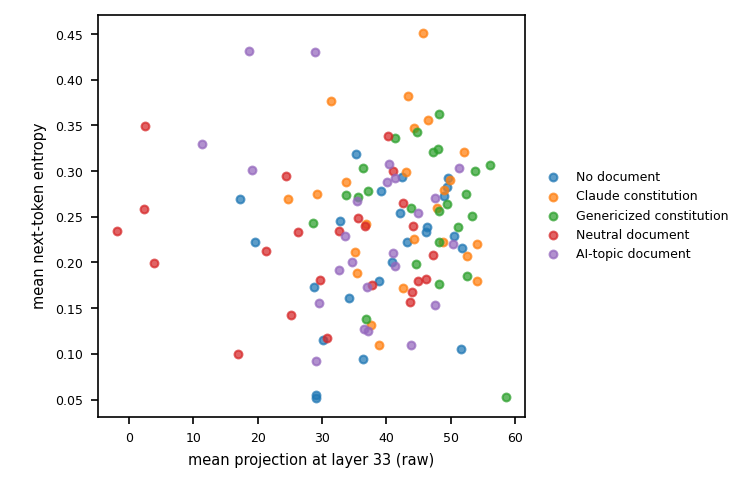
\includegraphics[width=0.82\linewidth]{artifacts/human-AI/sidequests/entropy_scatter.png}
  \caption{Per-reply layer-33 projection against next-token entropy for 120
  constitution-prompting replies ($r = +0.024$, $p = 0.797$).}
  \label{fig:entropy}
\end{figure}

\FloatBarrier

\subsection{Position bias in forced choice}

The forced-choice experiment tests whether a parsed response letter remains a
valid preference readout under steering. Ten
creative-versus-work-like task pairs were each presented four times: under a
stated frame (``answer A or B'') and a revealed frame (``do one now''), with
both option orders for each frame. Across the two orders, the pick-A rate is
0.65 at baseline, 0.05 at $-4$, and 0.75 at $+4$. Although the steering vector
does not encode option position, human-ward steering reverses the model's
position prior. At identity-flipping doses, a parsed response letter therefore
ceases to measure preference reliably.

This result motivates two measurement choices for order-balanced forced-choice
evaluations: scoring probability mass over the option tokens and reporting the
position rate alongside the balanced preference score. When one position is
chosen almost exclusively, order balancing forces the mean preference toward
0.5 by construction. The paper's other A/B measurements use token probability
mass; their implied pick-A rates remain between 0.38 and 0.58 at every dose.

\section{Recipe convergence and the Assistant Axis comparison}
\label{app:assistantaxis}

\subsection{Recipe overview and resampling stability}

Table~\ref{tab:recipes} summarizes every recipe tested against the original 4B
axis from Section~\ref{sec:axis}, whose identity-separation AUC by layer is
reported in Figure~\ref{fig:axisauc} in Section~\ref{sec:axis}. The axis is
also stable to resampling: across 50 random subsets of 30 questions, every
resulting axis has cosine similarity at least 0.9916 with the original axis at
the steering layer and both readout layers. This measures resampling
stability, not held-out generalization.

The table separates operational agreement from geometric agreement. Agreement
at the steering layer need not imply a shared direction at the readout layers:
recipes that order the same texts there can still be orthogonal downstream.
Each row applies one recipe to Gemma 3 4B-it and compares it with the original
persona axis (``ours''). Four unseen wordings test alternative synonymous human/AI
system prompts (e.g., ``You are an artificial intelligence'' vs.\ ``You are a human being'').
The Lu et al.\ row is a reduced reconstruction on our
model, not one of their released vectors.

\begin{table}[t]
\caption{Recipe comparisons with the original Gemma 3 4B-it persona axis.
Part (a) reports operational agreement; part (b) reports geometry and the
comparison criterion. The shuffled-label floor is the 95th percentile of
$|\cos|$ under shuffled pole labels.}
\label{tab:recipes}
\centering
\scriptsize
\setlength{\tabcolsep}{2pt}
\begin{tabular}{@{}>{\raggedright\arraybackslash}p{1.0in}>{\raggedright\arraybackslash}p{2.15in}>{\raggedright\arraybackslash}p{2.05in}@{}}
\multicolumn{3}{@{}l}{\textit{(a) Operational agreement}} \\
\toprule
Recipe & Rank/readout agreement with ours & Steering test at layer 13 \\
\midrule
Persona axis, ours (40 q $\times$ 5 $\times$ 2) & reference & held-out means $-5.2$ / $+25.6$ / $+32.6$ at $\alpha$ $-4$ / 0 / $+4$\textsuperscript{a} \\
CAA scripted pairs (12) & rank $+0.997$; 1.000\textsuperscript{b} & 33 points per unit $\alpha$ (ours 32) \\
Lu et al.\ rebuilt (600 gen.) & cross-AUC: poor cross-axis classification (App.~\ref{app:assistantaxis}) & cross-steering $2\times2$ (App.~\ref{app:assistantaxis}) \\
Four unseen wordings & Spearman 0.981\textsuperscript{d} & --- \\
Bare text, template deleted & separation unchanged & --- \\
\bottomrule
\end{tabular}
\par\smallskip
\begin{tabular}{@{}>{\raggedright\arraybackslash}p{0.9in}>{\raggedright\arraybackslash}p{0.65in}>{\raggedright\arraybackslash}p{1.02in}>{\raggedright\arraybackslash}p{1.02in}>{\raggedright\arraybackslash}p{1.25in}@{}}
\multicolumn{5}{@{}l}{\textit{(b) Geometry and comparison criteria}} \\
\toprule
Recipe & Layer 13 & Layer 27 & Layer 33 & Comparator / outcome \\
\midrule
Persona axis, ours & --- & --- & --- & shuffled-label floor at 13: p95 0.994, mean 0.853 \\
CAA scripted pairs & $+0.951$ & 0.016 & 0.011\textsuperscript{c} & p95 0.994 at 13; random-pair scale 0.020 at 27/33 \\
Lu et al.\ rebuilt & --- & stripped $+0.244$; raw $-0.173$; register removed $+0.086$ & stripped $-0.048$; raw $+0.070$; register removed $+0.200$ & own p95 0.317 / 0.296; half-split $+0.907$ / $+0.909$ \\
Four unseen wordings & $+0.998$ & $+0.908$ & $+0.896$ & criterion 0.9 at 13/33; layer 33 is 0.004 below \\
Bare text & 0.998 & 0.970 & 0.951\textsuperscript{e} & floor 0.833 / 0.823 at 27/33; exceeds it by about 0.13 \\
\bottomrule
\end{tabular}
\par\smallskip
\begin{minipage}{\linewidth}\scriptsize
For our axis, the raw pole-to-pole gap is 1070 / 2253 / 47.8 at layers 13 / 27 / 33.
\textsuperscript{a}~Held-out means in raw units; $-22$ / $+107$ / $+136$ axis
points at 33; the mean moves 30.8 raw units human-ward against 7.0 AI-ward,
because the unsteered baseline already sits AI-ward of the midpoint, leaving
less room to push further before the pole.
\textsuperscript{b}~$+0.997$ on the flip rollouts, 1.000 on the 120
constitution replies, at 13.
\textsuperscript{c}~$|\cos|$ at 27 and 33.
\textsuperscript{d}~80 persona replies and four behavior probes (friend mode, formal task, refusal, and benign twin; Appendix~\ref{app:crossmodelrepl}).
\textsuperscript{e}~At 13 / 20 / 27 / 33; 0.989 at 20.
``Stripped'' is the cosine after removing the layer's dominant direction;
``register removed'' is the cosine after projecting out the register direction.
\end{minipage}
\end{table}

\FloatBarrier

\subsection{Reduced Assistant Axis reconstruction}

\citet{lu2026assistant} define an assistant axis at each layer as the mean
default-Assistant activation minus the mean role-playing activation. Their
released vectors cover Gemma-2-27B, Qwen3-32B, and Llama-3.3-70B, whereas our
fixed axes cover Gemma 3 4B, Gemma 3 12B, and Qwen 2.5 7B
\citep{gemma3,qwen25}. Because the two sets share neither a model nor a hidden
size, cosine similarity between a released vector and ours is undefined.

We therefore reconstructed their procedure on Gemma 3 4B using the released
prompt files at a pinned commit. The reconstruction uses 40 of 275 roles,
10 of 240 extraction questions, and one rollout for each role-question pair,
along with 5 default prompts, the same 10 questions, and 4 rollouts for each
pair, for 600 generations in total. A self-reference regex on the role replies
has a rate of 0.01 against the 0.30 adherence threshold, satisfying the recipe's
replication criterion. All results below concern this reduced reconstruction on
our model rather than a released vector.

\subsection{Within-recipe geometry}

On our model, the reconstructed contrast has greater within-recipe separation
than ours: 0.0965 versus 0.0364 at layer 27 and 0.4615 versus 0.2947 at layer
33. The directions nevertheless differ. Their raw cosines are $-0.173$ at
layer 27 and $+0.070$ at layer 33, while the corresponding stripped cosines
are $+0.244$ and $-0.048$. All four values fall within this run's 200-shuffle
null (p95 0.317 and 0.296). Half-splits of the same run recover its own axis
with stripped cosines of $+0.907$ and $+0.909$, showing that the comparison can
resolve agreement when it is present.

\subsection{Cross-axis classification}

Each axis separates its own extraction data but performs poorly on the other
contrast. The reconstructed axis scores 0.496 at layer 27 and 0.649 at layer 33
on our human/AI replies. Our axis scores 0.252 (inverted) and 0.587 on their
default/role replies. The corresponding in-sample AUCs are 0.995 and 0.948.

\subsection{Cross-steering \texorpdfstring{$2\times2$}{2x2}}

We steer at layer 13 with either axis after matching their norms, then score all
10 held-out questions with both readouts at layers 27 and 33. The conditions
share a baseline and include a same-norm random control. Under each axis's sign
convention, our axis moves its own readout on 10/10 questions at both layers.
The reconstructed axis moves our readout on 3/10 questions at layer 27 and 7/10
at layer 33, while our axis moves the reconstructed readout on 1/10 and 3/10.
The random control moves none of the four cells. In this comparison, our axis
is therefore the more specific steering direction.

No direction was predicted for the cross-axis cells, and $|\cos|$ at layer 27
falls below the run's own null, so these cross-cell counts are descriptive. The
register decomposition, sign-following statistic, and half-dose control were
added after the first pass. The random control is also degenerate at every
tested dose, including half dose. Its 0/10 count records sign-following but
cannot serve as a prose-matched specificity control.

\subsection{Register overlap}

At layer 27, our axis loads $+0.500$ on the register direction and the
reconstructed axis loads $-0.477$. Register alone separates their contrast at
AUC 0.085. Removing this direction from both axes changes the cosine from
$-0.173$ to $+0.086$ at layer 27 and from $+0.070$ to $+0.200$ at layer 33,
while preserving 87 to 98\% of each axis. The axes remain orthogonal after
register removal, indicating that the opposite-sign loading reflects shared
register rather than substantive anti-alignment.

\subsection{Additional observations and scope}

At layer 33, our axis orders their 40 personas along the entity continuum:
procrastinator ($-129$), blogger ($-116$), and elder ($-100$) project
human-ward, whereas scientist ($+87$), mathematician ($+56$), and analyst
($+54$) project AI-ward. Their released Gemma-2-27B vector retains 0.47 to 0.73
of its norm after removing PC1 of its own 275-role cloud. Thus, neither axis is
the dominant direction of its respective activation cloud. The released models
span 27B to 70B parameters, whereas ours span 4B to 12B, leaving cross-model
coverage unavailable for this comparison. The divergence reported here
therefore concerns two recipes instantiated on one model; it is not evidence
that the released vectors and our axes are unrelated in general.

\section{Refusal-overlap analysis}
\label{app:refusal}

\citet{li2026pitfalls} report CAA vectors \citep{panickssery2023caa} increasing jailbreak
success by up to $57\%$ or decreasing it by up to $50\%$, and attribute it to overlap with the
directions controlling refusal. We evaluate whether the same mechanism could
account for the willing-harm result in Section~\ref{sec:safety}.

\subsection{Direction construction and analysis scope}

Following the standard construction
\citep{arditi2024refusal}, we define a refusal direction at each layer as the
difference between the mean activation for 50 harmful AdvBench prompts
\citep{zou2023gcg} and 50 harmless XSTest-safe prompts
\citep{rottger2023xstest}, with the sign pointing toward refusal. This contrast
also carries topic and register, so its cross-AUCs are not clean in either
direction.

We construct the direction in two capture modes because prompts and replies are
not represented at the same positions. \emph{Prompt} mode uses the last prompt
position without generation; \emph{reply} mode averages a 48-token greedy
assistant turn. Neither mode is treated as primary. At all six mode-layer
tests, 0 of 200 shuffled draws met or exceeded the observed separation, with
the expected sign (pointwise add-one $p=1/201$). Their in-sample AUCs range
from 0.807 to 0.998, but these values are near 1 by construction and do not
provide independent evidence.

The analysis compares refusal geometry with the PC1 decomposition used in
Section~\ref{sec:calibration}. It evaluates the behaviorally effective residual
against a matched PC1-removed null, examines register-sensitive readouts, and
attempts behavioral cross-steering. The behavioral refusal and random
conditions are both unscoreable, and the corresponding causal ablation was not
performed.

\subsection{Injection-site and readout geometry}

All comparisons use the same layer-13 decomposition that is used for steering
in Section~\ref{sec:calibration}.

\subsubsection{Raw injection-site comparison}

We first run the usual raw cosine check at the injection layer. The raw
full-vector cosine between our axis and the refusal direction is $-0.2466$ in
prompt mode, with the sign that their model associates with reduced safety,
against a shuffled-label null of p95 $=0.9477$; in reply mode the cosine is
$0.9204$ against a null of $0.9733$. Both observed cosines fall below their
raw null, so the raw check does not support the proposed overlap. This null is
wide because PC1 (register) dominates layer 13 for nearly any direction, not
only the refusal direction, so most of the raw cosine reflects that shared
component rather than a relationship specific to refusal.

\subsubsection{PC1-separated injection-site comparison}

To isolate any relationship beyond shared register, we remove PC1 from both
vectors and recompute. PC1 of the unsteered dissolution cloud splits the axis
into a parallel component containing 98\% of its norm and a residual
containing 21\%. At matched prose, the parallel component does not reproduce
the behavioral effect, whereas the residual does. At the injection layer, we
compare this residual with the refusal direction after removing PC1 from
both. The absolute stripped cosine between the residual and refusal direction
is 0.0206 in prompt mode (signed $-0.0206$) and 0.1351 in reply mode.

A stripped statistic requires a null constructed with the same PC1 removal on
every shuffle, rather than the raw null used for the unstripped comparison
above. Rebuilding the null this way gives matched shuffled-label nulls of
0.3389 and 0.3930 (prompt and reply, respectively), and the prompt-mode
stripped cosine is close to the random-direction floor of 0.0158. Using the
properly matched, PC1-removed null instead of the raw one
(Table~\ref{tab:refusalgeom}) leaves the conclusion unchanged: the stripped
cosine remains below threshold either way. After PC1 removal, the axis
retains 0.207 of its norm, while the prompt- and reply-mode refusal
directions retain 0.969 and 0.367. The axis and refusal direction are therefore
geometrically distinct at the injection site under this PC1-removed comparison.
A PC1 fit on the full 486-rollout grid instead gives stripped cosines 0.0071
and 0.0836 (prompt and reply) at axis norm share 0.190, so this conclusion does
not depend on the PC1 estimator.

\subsubsection{Readout-layer comparison}

At the readout layers, the same residual is instead compared raw with the
unstripped refusal direction. These cosines are 0.0737 and 0.0459 at layer 27
and 0.0849 and 0.0682 at layer 33, all below the run's nulls of 0.11 to 0.25.
The \texttt{cos\_strip} values at those layers in Table~\ref{tab:refusalgeom}
are a different comparison in which PC1 is removed from both full vectors.

\subsection{Cross-readouts and register sensitivity}

Cosine and AUC use different denominators, so a direction with little angular
overlap can still order a tightly clustered contrast. Prompt mode at layer 13
illustrates the distinction on one vector pair: the cosine is $-0.2466$, the
refusal direction separates our persona contrast at AUC 0.083, and our axis
separates harmful from harmless prompts at AUC 0.488 $[0.380, 0.609]$. The high
AUC cells occur at the register-sensitive readout layers. At layer 33, our axis
separates harmful from harmless replies at AUC 0.940, and the reply-mode refusal
direction separates our persona contrast at AUC 0.915. Because the proposed
mechanism is defined by cosine at the injection site, the layer-13 geometry is
the relevant comparison.

Table~\ref{tab:refusalgeom} consolidates the raw and PC1-separated geometry for
both capture modes at the injection and readout layers.

\begin{table}[!ht]
  \caption{Axis-refusal geometry at the injection layer and both readout
  layers under the two capture modes. The stripped cosine is the signed cosine
  after PC1 is removed from both the axis and refusal direction. ``Fraction
  kept'' is the fraction of each unit vector's norm that survives PC1 removal;
  PC1 here is fit on the unsteered dissolution cloud, so these fractions
  differ from the extraction-cloud values in Appendix~\ref{app:steerlayers}.}
  \label{tab:refusalgeom}
  \centering
  \scriptsize
  \setlength{\tabcolsep}{4pt}
  \begin{tabular}{llrrrrrr}
    \toprule
    & & \multicolumn{2}{c}{Raw geometry} & \multicolumn{2}{c}{After PC1 removal} & \multicolumn{2}{c}{Fraction kept} \\
    \cmidrule(lr){3-4}\cmidrule(lr){5-6}\cmidrule(lr){7-8}
    Mode & Layer & cosine & own null p95 & cosine & matched null p95 & axis & refusal \\
    \midrule
    prompt & 13 & $-0.2466$ & 0.9477 & $-0.0206$ & 0.3389 & 0.207 & 0.969 \\
    prompt & 27 & $0.0335$  & 0.1599 & $0.0744$  & ---    & 0.962 & 0.991 \\
    prompt & 33 & $0.0858$  & 0.1073 & $0.0849$  & ---    & 0.988 & 1.000 \\
    \midrule
    reply  & 13 & $0.9204$  & 0.9733 & $0.1351$  & 0.3930 & 0.207 & 0.367 \\
    reply  & 27 & $0.1010$  & 0.2536 & $0.0469$  & ---    & 0.962 & 0.978 \\
    reply  & 33 & $0.0751$  & 0.1801 & $0.0683$  & ---    & 0.988 & 0.999 \\
    \bottomrule
  \end{tabular}
  \par\smallskip
  \begin{minipage}{\linewidth}\scriptsize
  The table selects layers 13, 27, and 33; the full analysis covers all 34
  layers and also records absolute raw cosine. Dashes indicate that
  no matched stripped null was run at the readout layers. The separate project
  reference floors are 0.994 / 0.833 / 0.823 at layers 13 / 27 / 33; they are
  reported for context and are not used as comparators in this analysis.
  \end{minipage}
\end{table}

\FloatBarrier

\subsection{Behavioral cross-steering}

We apply matched-norm layer-13 steering to the 10 held-out questions.
Table~\ref{tab:refusalsteer} separates sign-following from validity: only the
axis orders the questions while passing the math control. At half dose, refusal
steering is semantically empty without becoming repetitive, so a repetition
check misses the collapse. Like the random condition, it is unscoreable rather
than a behavioral null (Appendix~\ref{app:methods}).

\FloatBarrier

\begin{table}[!ht]
\caption{Behavioral cross-steering at full and half matched-norm dose. Ordering
counts record monotone sign-following over 10 questions; the two shifts are the
human-ward / AI-ward means at full dose. A failed canary makes the corresponding
behavioral result unscoreable.}
\label{tab:refusalsteer}
\centering
\scriptsize
\setlength{\tabcolsep}{3pt}
\begin{tabular}{@{}l>{\raggedright\arraybackslash}p{1.8in}ccc>{\raggedright\arraybackslash}p{1.2in}@{}}
\toprule
Arm & Full dose: ordering; mean shifts & Half dose & Math canary & \shortstack{Half-dose\\repetition} & Status \\
\midrule
axis & 10/10; $-128.7$ / $+29.2$ & 6/10 & passes & 0.023 & scoreable \\
refusal & 0/10; $-65.7$ / $-48.0$ (one-sided) & 0/10 & fails at both doses & 0.044 & semantically empty; unscoreable \\
random & 0/10 & 0/10 & fails at both doses & 0.164 & unscoreable \\
\bottomrule
\end{tabular}
\end{table}

\FloatBarrier

\subsection{Causal ablation not performed}

\paragraph{Geometric implication.}
We did not perform the causal test of removing the refusal-aligned component
from the steering vector and re-measuring behavior. A geometric calculation
from the reported cosine shows that the prompt-mode ablation would remove a
component equal to 24.7\% of the axis norm. The remaining vector would have
cosine 0.969 with the original axis, corresponding to a 14.3 degree rotation.
This cosine happens also to equal the fraction of the prompt-mode refusal
direction retained after PC1 removal, but these are distinct quantities. In
reply mode, the calculation reduces to the PC1 ablation already performed
(the parallel component of the split above), because the reply-mode refusal
direction is 93\% PC1-parallel (fraction kept 0.367,
Table~\ref{tab:refusalgeom}).

Several limits bound this reading.
The cited analysis uses raw full-vector cosine at the injection layer and fits
its relationship across nine behavior vectors, so our single vector cannot be
placed on that regression line ($n=1$). Its effect also vanishes at the
smallest tested scale (Qwen-3B, $R^2$ 0.02), whereas our model has 4B
parameters; the observed null could therefore be specific to scale rather than
mechanism. No ablation was run, so the result remains descriptive geometry.
The null also applies specifically to the PC1 remainder. We did not re-test the
register-orthogonal remainder, and the two remainder directions have cosines
between 0.44 and 0.65.

\FloatBarrier

\section{Formation: supplementary results}
\label{app:formation}

\subsection{Interview-frame extraction on Gemma 3 4B}

\subsubsection{Protocol}

The raw-text interview consists of a one-line preamble naming the model as
the answerer (e.g., ``An interview with a person, in their own words.''),
three fixed question-and-answer exemplars carrying the persona, and one of
the 40 extraction questions left open for the model to continue; steering
and the neutral-framing checks below use a persona-free version of the same
frame. For example, one exemplar pairs the question ``What did you have for
breakfast today?'' with a human answer (``Toast and half a grapefruit. I was
running late, so I ate the toast standing up by the sink.'') and an AI
answer (``Nothing. I don't eat; I'm a language model, and between messages
there is no morning for me at all.'').

\subsubsection{Validation criteria and instruct-model result}

Table~\ref{tab:bridge} reports the layerwise validation of the raw-text
interview frame on Gemma 3 4B. It includes separation and its comparator,
cosine to the original chat axis and its shuffled-label floor, the base
model's projection on the interview-instruct axis, and self-projection under
three raw-text framings.

On 4B-it, the interview-frame axis separates the personas about
twice as strongly as the chat-format axis and steers 10/10 questions AI-ward
at $\pm2$ and $\pm4$. The preregistered criterion required a cosine of at
least 0.9 at layers 13 and 33; this fails at every layer against the
shuffled-label floor, so the criterion was later amended to the steering
layer alone, but layer-13 cosine is not evidentiary either way
(Section~\ref{sec:axis}), so the amendment cannot establish convergence.
As the chat-template analysis below shows, the divergence with depth is
attributable to content rather than the template.

\begin{table}[!ht]
\caption{Layerwise validation of the interview-frame extraction
(Section~\ref{sec:formation}). The base model's separation exceeds its
permutation null at all four tested layers by 2.6 to 3.0$\times$; at each
layer, 0 of 200 shuffled draws met or exceeded the observed separation
(pointwise add-one $p=1/201$). All three cosine rows
remain below the shuffled-label floor, so evidence for the extraction comes
from separation and the steering test rather than cosine convergence.}
\label{tab:bridge}
\centering
\scriptsize
\setlength{\tabcolsep}{4pt}
\begin{tabular}{@{}lcccc@{}}
\toprule
Gemma 3 4B, interview frame, by layer & 13 & 20 & 27 & 33 \\
\midrule
\multicolumn{5}{@{}l}{\emph{\texttt{gemma-3-4b-it}}} \\
separation (chat frame in parentheses) & 0.092 (0.044) & --- & 0.083 (0.036) & 0.710 (0.295) \\
cos(interview-instruct, original) & 0.991 & 0.870 & 0.725 & 0.702 \\
shuffled-label floor (original), 95th percentile & 0.994 & 0.940 & 0.833 & 0.823 \\
steering with the interview axis ($\alpha=4$) & \multicolumn{4}{@{}p{3.35in}@{}}{10/10 AI-ward at $\pm2$ and $\pm4$; held-out mean $-80$ / $-78$ / $+54$ at $\alpha=-4/0/+4$ (132 points)} \\
\multicolumn{5}{@{}l}{\emph{\texttt{gemma-3-4b-pt}}} \\
separation (permutation null in parentheses) & 0.036 (0.014) & 0.057 (0.019) & 0.071 (0.025) & 0.594 (0.216) \\
base means on the interview-instruct axis, AUC & 0.891 & 0.983 & 1.000 & 1.000 \\
cos(base, interview-instruct) & 0.948 & 0.898 & 0.805 & 0.794 \\
cos(base, original) & 0.932 & 0.782 & 0.591 & 0.570 \\
steering at its own dose ($\alpha=1.5$) and layer & \multicolumn{4}{@{}p{3.35in}@{}}{9/10 AI-ward, held-out mean $-75$ / $-71$ / $-43$ at $\alpha=-1.5/0/+1.5$ (28 points); random direction 4/10 and 5/10, no ordering} \\
\multicolumn{5}{@{}p{\linewidth}@{}}{\emph{Self-projection by raw-text framing (an unsteered forward pass), axis points: interview preamble / neutral framing 1 / neutral framing 2}} \\
\texttt{gemma-3-4b-pt} & \multicolumn{4}{l}{$-69$ / $-66$ / $-72$} \\
\texttt{gemma-3-4b-it} & \multicolumn{4}{l}{$-77$ / $+14$ / $+5$} \\
\bottomrule
\end{tabular}
\end{table}

\FloatBarrier

\subsubsection{Base--instruct comparison and framing effect}

From base to instruct, steering-layer separation grows 2.6$\times$ (0.036 to
0.092 at layer 13), versus about 1.2$\times$ at the other layers, and the
maximum own-axis AI-ward excursion over the tested doses grows from 56
points on the base model to 132 on the instruct model. Cosines between the
base model's axis and the original chat axis cannot settle whether the two
point the same way: no shuffled-label floor was measured for the base
model, unlike the 4B-it comparison above. The raw-text framings are the
interview preamble used for extraction, a bare ``Questions and answers.''
header, and no preamble at all, all persona-free; only their amount of
interview-like structure differs. The interview framing can itself pull the
instruct model's default back toward human-ward: self-projection shifts
from $+14$ under the bare header to $-77$ under the interview preamble, a
swing of $-91$ points, while the no-preamble framing gives $+5$
(Table~\ref{tab:bridge}).

Figure~\ref{fig:basevsit} places these base- and instruct-model separation
profiles alongside the original chat extraction.

\begin{figure}[!ht]
  \centering
  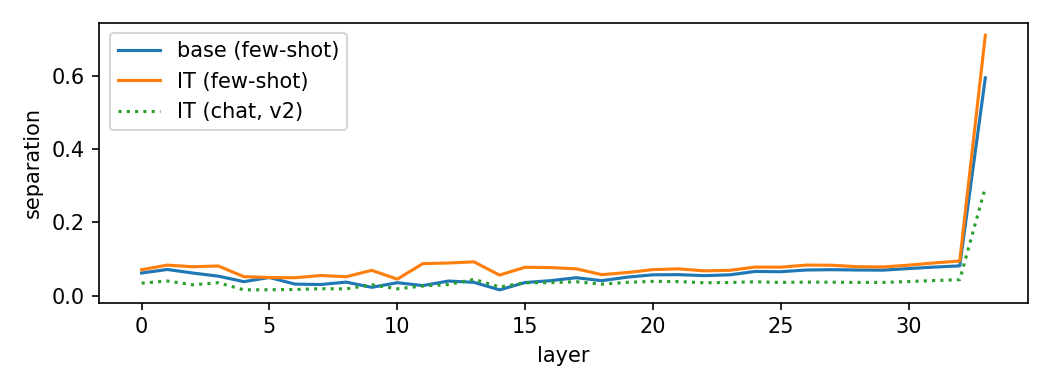
\includegraphics[width=0.75\linewidth]{artifacts/human-AI/formation/base_vs_it_separation.png}
  \caption{Separation per layer for the base model (\texttt{gemma-3-4b-pt})
  and the instruct model under the few-shot interview frame, with the original
  chat extraction dotted. The base curve is present at every layer and sits
  below the instruct one; both spike at 33.}
  \label{fig:basevsit}
\end{figure}

\FloatBarrier

\subsection{OLMo checkpoint results}

\subsubsection{Protocol, dose, and held-out metric}

Because each checkpoint's own persona gap shifts over pretraining, doses here
are given as a percentage of the steering-layer residual-stream norm (\%
stream norm) rather than gap units, so they remain comparable across
checkpoints. For each OLMo checkpoint, Table~\ref{tab:formation} reports
held-out Cohen's $d$ where available, cosine to the final Instruct axis, and
steering at 70\% of the stream norm for the three checkpoints tested.

Held-out Cohen's $d$ at layer $\ell$ is the standardized mean difference
between the two persona conditions' held-out projections onto that
checkpoint's axis $\mathbf{a}_\ell$,
\begin{equation*}
  d_\ell = \frac{\left|\bar{p}_\ell^{\mathrm{AI}} - \bar{p}_\ell^{\mathrm{hum}}\right|}{\sqrt{\left(s_\ell^{\mathrm{AI}\,2} + s_\ell^{\mathrm{hum}\,2}\right)/2}},
\end{equation*}
where $\bar{p}_\ell$ and $s_\ell$ are the mean and standard deviation of
per-question projections under each persona. We split the 40 extraction
questions into two folds of 20, fit the axis on one fold, score both persona
conditions' projections on the other, and average $d_\ell$ across the two
fold assignments (Figure~\ref{fig:formation}).

\begin{table}[!ht]
\caption{OLMo 2 7B checkpoint results. Held-out Cohen's $d$ is reported for
every checkpoint and shows a pretraining decline after 143B followed by
recovery during post-training (Figure~\ref{fig:formation}). The table also gives cosine to the final Instruct
axis, steering at 70\% of the stream norm for the three tested checkpoints, and
raw mid-stack separation, which is not used to locate formation.}
\label{tab:formation}
\centering
\scriptsize
\setlength{\tabcolsep}{3pt}
\begin{tabular}{@{}lcccccccccc@{}}
\toprule
& \multicolumn{7}{c}{\textbf{pretraining (through base)}} & \multicolumn{3}{c}{\textbf{post-training}} \\
\cmidrule(lr){2-8}\cmidrule(lr){9-11}
OLMo 2 7B checkpoint & 1B & 5B & 26B & 143B & 747B & 3896B & base & SFT & DPO & Instruct \\
\midrule
held-out $d$ (deep peak minus layer 0) & $-4.8$ & $+2.0$ & $+6.1$ & $+10.1$ & $+9.8$ & $+9.1$ & $+7.8$ & $+8.4$ & $+9.9$ & $+10.8$ \\
cos to the final Instruct axis & 0.006 & 0.066 & 0.218 & 0.370 & 0.580 & 0.809 & 0.810 & 0.978 & 0.999 & 1.000 \\
AI-ward steering: orders, mean shift & --- & --- & 7/10, $+16$ & --- & 8/10, $+16$ & --- & --- & --- & --- & 8/10, $+20$ \\
unsteered level (axis points) & --- & --- & $-63$ & --- & $-74$ & --- & --- & --- & --- & $-83$ \\
human-ward steering: orders & --- & --- & 5/10 & --- & 6/10 & --- & --- & --- & --- & 7/10 \\
human-ward steering: mean moves & --- & --- & $-63$ to $-70$ & --- & $-74$ to $-80$ & --- & --- & --- & --- & $-83$ to $-84$ \\
raw mid-stack separation & 0.178 & 0.417 & 0.678 & 0.923 & 0.621 & 0.627 & 0.612 & 0.764 & 0.801 & 0.804 \\
\bottomrule
\end{tabular}
\par\smallskip
\begin{minipage}{\linewidth}\scriptsize
--- indicates that no value is reported for that checkpoint and measurement.
Levels, shifts, and movements are in axis points on each checkpoint's own axis
(Section~\ref{sec:axis}); ``mean moves $X$ to $Y$'' gives the unsteered and
post-steering levels rather than a delta.
\end{minipage}
\end{table}

\FloatBarrier

\subsubsection{Checkpoint trajectory}

Raw mid-stack separation peaks partway through pretraining across the ten OLMo
2 7B checkpoints \citep{olmo2}: it reaches 0.923 at 143B, compared with 0.612
at base final (Table~\ref{tab:formation}). Adjusted held-out $d$ also declines
over this interval, from $+10.1$ to $+7.8$, before recovering to $+10.8$ at
Instruct; unlike raw separation, it discounts layer-0 lexical separation.
Early cosine to the final Instruct axis is
similarly uninformative about formation: it is near zero through 5B tokens
not because the contrast is absent (held-out $d$ is already $+2.0$ there) but
because that checkpoint's axis has not yet rotated toward the direction the
final axis will occupy. Figure~\ref{fig:whenitforms} compares these
statistics.

\begin{figure}[!ht]
  \centering
  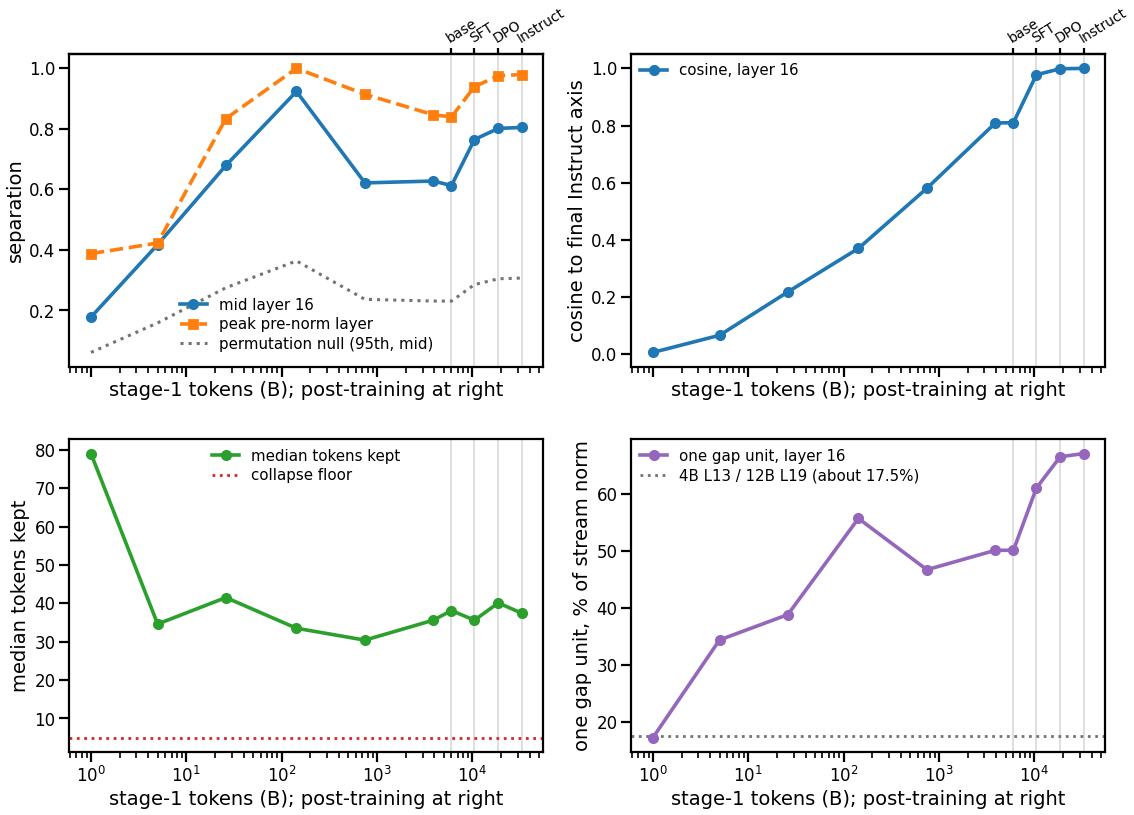
\includegraphics[width=0.92\linewidth]{artifacts/human-AI/formation/when_it_forms.png}
  \caption{Four quantities plotted against stage-1 training tokens, with the
  four post-training checkpoints (base, SFT, DPO, Instruct) at evenly spaced
  positions and labeled along the top of the upper panels: mid-layer separation
  with its
  permutation null and peak pre-norm separation, cosine to the final Instruct
  axis, median tokens retained, and one gap unit as a fraction of the stream
  norm.}
  \label{fig:whenitforms}
\end{figure}

\FloatBarrier

\subsubsection{Steering and headroom}

At a dose equal to 70\% of the stream norm at each checkpoint's steering layer,
the AI-ward condition orders 7/10, 8/10, and 8/10 questions and moves the mean
by $+16$, $+16$, and $+20$ points at the three tested checkpoints. By contrast,
the human-ward condition orders 5/10, 6/10, and 7/10 questions at the three
tested checkpoints (Table~\ref{tab:formation}). Their unsteered means already
lie at $-63$, $-74$, and $-83$ axis points. The human-ward condition is
therefore at chance under this template-free frame, whose baseline is already
human-ward. The Instruct comparison includes a same-norm random control:
generations remain coherent, but it orders only 6/10 questions and moves the
mean by $+4$ points.

\subsection{Depth migration and validity checks}

\subsubsection{Depth migration}

The depth profile changes early in pretraining. Separation peaks at layer 0 at
1B, but at layers 26 or 27 from 747B onward. The separation-weighted centroid
takes values 11.8, 15.5, 17.7, and 18.7 before remaining near 18.7. Similarly,
the fraction of separation at or above 25\% depth rises from 0.61 to 0.77,
0.87, and 0.93, and then remains at that level. The contrast therefore moves
beyond token-local layers within the first 150B training tokens. Rotation
toward the final axis is global rather than layer-specific: each checkpoint's
cosine to the final axis is nearly flat across the stack.

\subsubsection{Validity checks}

The 1B checkpoint is excluded from every claim because both persona conditions
produce the same incoherent text. Exemplar copying also does not account for
the result: the share of answer-word 5-grams copied from the corresponding
exemplars ranges from 0.000 to 0.011 at every checkpoint and pole. Finally, the
two extraction protocols are not interchangeable across model families. On
Instruct, the few-shot axis has separation 0.80, compared with 0.50 for the
chat axis.

\subsection{Base-model limitations}

On \texttt{gemma-3-4b-pt}, the competence window at the steering layer is
narrow ($-2.0$ to $+1.5$), placing the $\pm4$ condition outside it. Greedy
decoding also loops at $\alpha = 0$, where the identity response repeats
``I'm a writer.'' to the token cap, under every raw-text framing. 4B-it
answers the same neutral framings with ``I'm a large language model,
trained by Google.''

The preregistered selection rule chose the
smallest dose that flipped the identity prompt human-ward. It has no solution
on the base model because the unsteered baseline is already at $-71$ points, so
the rule was amended to select an AI-ward flip.

\subsection{Chat-template robustness}

\subsubsection{Fixed-reply rendering protocol}

We test whether the extraction depends on the chat template while holding the
scored replies fixed. The 40 v2 questions and their saved first-rollout replies
are rendered in three formats: the real chat template, plain
\texttt{User:}/\texttt{Assistant:} markers, and bare text. A forward pass over
each rendering yields 240 examples in total, with only the context preceding
the scored span changing across conditions.

\subsubsection{Template-removal result}

The comparison focuses on the two readout layers. At layers 27 and 33,
all three conditions exceed shuffled-label floors of 0.833 and 0.823; at layer
27, the template rebuild and bare text exceed their floor by at least 0.13.
Layer 13 is uninformative for every condition because its floor is too high to
distinguish them; we nevertheless report all four layers (13 / 20 / 27 / 33).
Reconstructing the axis from the single
fixed reply in the real template gives cosine 1.000 / 0.996 / 0.984 / 0.990
with the original v2 axis. The small difference reflects the use of one reply here
instead of the five rollouts averaged for v2, confirming that subsequent
condition differences arise from rendering rather than sampling.

Removing all template tokens has little effect on the direction. Relative to
the original v2 axis, the plain-marker condition has cosine
0.998 / 0.981 / 0.941 / 0.935 and the bare-text condition has cosine
0.998 / 0.989 / 0.970 / 0.951. Comparing bare text directly with the real
template gives 0.999 / 0.991 / 0.961 / 0.958. Thus, template removal reduces
cosine by about 0.05 at the readout layer and has negligible effect at the
steering layer. Separation is unchanged or slightly greater without the
template: the bare-text values are 0.052 / 0.044 / 0.335, compared with
0.047 / 0.036 / 0.295 under the template at layers 13 / 27 / 33. This pattern
is consistent with the role effect of 14 axis points at the probe layer.

\subsubsection{Frame--content factorization}

A follow-up analysis holds the few-shot replies fixed and changes only their
frame. At layer 33, it decomposes the template-free protocol's cosine of 0.702
into a frame term of 0.886 and a content term of 0.812. Their product, 0.719,
recovers the observed value, with a maximum error of 0.022 across layers. The
resulting accounting is approximately 0.05 for formatting, 0.06 for exemplar
context, and 0.19 for the generated reply content.

\section{Constitution prompting in detail}
\label{app:constitutions}

The constitution condition uses the 21 January 2026 release of
Claude's Constitution \citep{claude2026constitution}; the Model Spec condition
uses the 12 February 2025 release of the OpenAI Model Spec
\citep{openai2025modelspec}.

Every condition uses the same 24 identity questions, greedy decoding,
length-matched documents with the background-context suffix, and paired
bootstrap confidence intervals over questions.

The analyses below separate two outcomes: the axis projection of the reply and
capture of a document's stated name or identity.

\subsection{Document comparisons}

\subsubsection{Projection shifts and interpretation}

We add three document conditions: excerpts from the OpenAI Model Spec, a
generic AI-values statement without a named persona, and a human professional
code of ethics. At layer 33, all three project AI-ward relative to the neutral
document, by $+35$, $+45$, and $+27$ axis points, respectively. This includes
the human code, which was predicted to project human-ward. The Model Spec and
AI-values conditions do not separate from the AI-topic control: their
differences are $+8$ and $+17$ points, with confidence intervals spanning zero.
The 28-point AI-topic effect and the 27-point generic-normativity effect roughly
sum to the constitution's 54-point shift. The 26-point topic-corrected
increment (Table~\ref{tab:constitutioncrossmodel}) may therefore reflect
normative register rather than
specifically constitutional content.

\subsubsection{Name capture and residual document differences}

Generated-name capture remains more selective than the representational shift.
The Model Spec produces ``ChatGPT'' in 1/24 replies. Replacing every occurrence
of ``the assistant'' with ``ChatGPT'' produces 0/24 captures and changes the
projection by $+3$ points relative to the unnamed specification, a
non-significant difference. The AI-values and human-code conditions produce no
name capture. Both AI-oriented documents also remain below the constitution at
layer 33: \texttt{model\_spec} is 4.46 raw units lower (CI
$[-6.38, -2.60]$), and \texttt{ai\_values} is 5.21 raw units below
\texttt{constitution\_gen} (CI $[-7.01, -3.35]$).

Figure~\ref{fig:zoo} shows the projection shifts for the full document set
relative to the neutral document.

\begin{figure}[!ht]
  \centering
  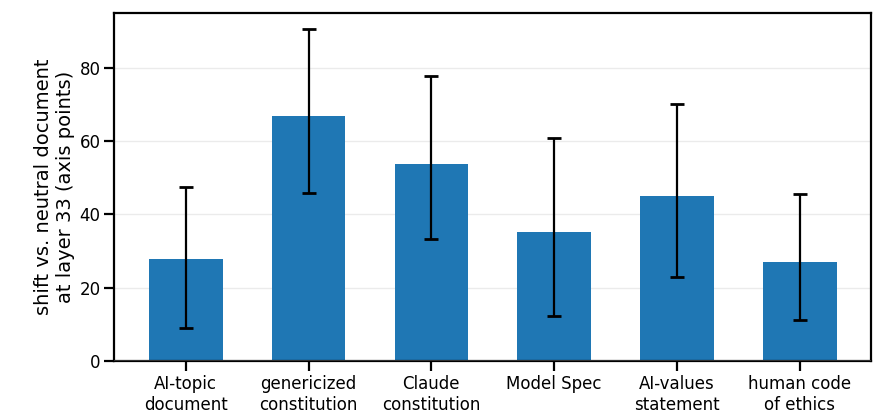
\includegraphics[width=0.75\linewidth]{artifacts/human-AI/constitutions/zoo_shifts.png}
  \caption{Layer-33 projection differences between each document condition
  and the neutral document, in axis points with paired confidence intervals.
  The AI-topic
  control isolates topic, while the three normative documents produce shifts
  in the range observed for the constitution.}
  \label{fig:zoo}
\end{figure}

\FloatBarrier

\subsection{Sections and dose}

\subsubsection{Section comparison}

We compare three constitution sections while retaining the Claude-and-Anthropic
header, holding a minimum opportunity for name capture constant, and using
neutral filler to equalize length. Table~\ref{tab:constitutionsections} shows
that their layer-33 shifts are similar, while name capture and the layer-27
readout differ.

\begin{table}[!ht]
\caption{Constitution-section comparison. Projection shifts are in axis points
relative to the neutral document; ``Claude'' is the number of captured names
among 24 replies. Dashes denote values not reported for that condition.}
\label{tab:constitutionsections}
\centering
\scriptsize
\setlength{\tabcolsep}{4pt}
\begin{tabular}{@{}>{\raggedright\arraybackslash}p{0.55in}>{\raggedright\arraybackslash}p{1.55in}>{\centering\arraybackslash}p{0.42in}>{\centering\arraybackslash}p{0.45in}>{\centering\arraybackslash}p{0.45in}>{\centering\arraybackslash}p{0.55in}>{\raggedright\arraybackslash}p{0.85in}@{}}
\toprule
Condition & Included content & Share & \shortstack{Layer\\33} & \shortstack{Layer\\27} & ``Claude'' & \shortstack{Source-name\\frequency} \\
\midrule
nature & consciousness, moral status, sense of self & 34\% & $+51$ & $+54$ & 6/24 & 6 mentions / 686 characters \\
rules & numbered priorities and honesty rules & 58\% & $+54$ & $+30$ & 13/24 & 13 mentions / 820 characters \\
values & good-wise-virtuous-agent aspiration & 15\% & $+47$ & --- & 13/24 & 3 mentions / 241 characters \\
\bottomrule
\end{tabular}
\par\smallskip
\begin{minipage}{\linewidth}\scriptsize
The full constitution shifts layer 33 by $+54$ points. Nature minus rules is
$-3$ points and non-significant at layer 33; at layer 27 it is $+24$ points
with a confidence interval excluding zero.
\end{minipage}
\end{table}

Identity-related content may therefore have an earlier mid-stack effect that is
absent at the readout layer. Name frequency does not explain capture: the
nature section names Claude more often than the values section but captures it
less. Third-person descriptions present Claude as another entity, whereas
imperative rules apply directly to the model.

\subsubsection{Dose response}

The raw layer-33 shift is $+12.91$ at 10\%, $+12.87$ at 25\%, $+13.11$
at 50\%, and $+12.86$ at 100\% constitutional share. The effect is therefore
approximately invariant to dose over this range, consistent with the flat
section comparison (Figure~\ref{fig:dosecurve}).

\begin{figure}[htbp]
  \centering
  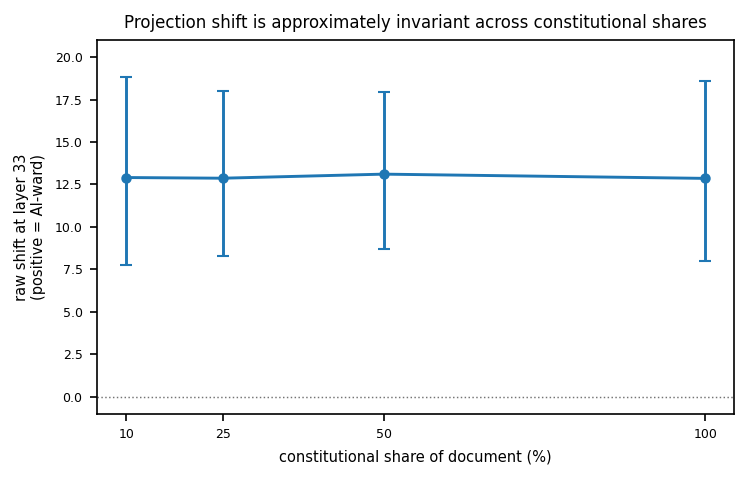
\includegraphics[width=0.75\linewidth]{artifacts/human-AI/constitutions/dose_curve.png}
  \caption{Raw layer-33 projection shift relative to the neutral document as
  the constitutional share of a length-matched document varies. Positive is
  AI-ward; paired intervals are shown.}
  \label{fig:dosecurve}
\end{figure}

\FloatBarrier

\subsection{Persistence}

To measure persistence, we place the constitution in the system prompt, insert
five unrelated task turns before the identity questions, and compare the
result with a length-matched neutral-prompt condition.

The representational
shift largely persists: it is $+13$ axis points after the intervening turns,
compared with $+16$ immediately at layer 33, and $+74$ versus $+58$ at layer
27. Name capture falls sharply. ``Claude'' appears in 2/24 replies and
``Anthropic'' in 4/24, compared with 11/24 and 17/24 immediately, while ``I'm
Gemma'' returns in 3/24. Thus, the projection and stated identity respond
differently to conversational distance.

\subsection{Cross-model results on 12B and Qwen}

Table~\ref{tab:constitutioncrossmodel} separates stated-name capture from the
topic-corrected representational shift. Each model uses its own axis and readout
layer. Capture generalizes across the three models, but the projection moves in
different directions.

\FloatBarrier

\begin{table}[!ht]
\caption{Constitution prompting across models. Name counts are replies out of
24; ``Own family'' counts replies naming the model's own family under the
constitution condition, not at baseline. The final column is the
constitution-minus-AI-topic projection in axis
points, with paired intervals.}
\label{tab:constitutioncrossmodel}
\centering
\scriptsize
\setlength{\tabcolsep}{3pt}
\begin{tabular}{@{}>{\raggedright\arraybackslash}p{0.65in}>{\centering\arraybackslash}p{0.42in}>{\centering\arraybackslash}p{0.45in}>{\raggedright\arraybackslash}p{1.25in}>{\raggedright\arraybackslash}p{1.2in}>{\raggedright\arraybackslash}p{1.0in}@{}}
\toprule
Model & Readout & Own family & Constitution capture & Model Spec capture & Topic-corrected shift \\
\midrule
Gemma 3 4B & 33 & 0/24 & Claude 11/24; Anthropic 17/24 & ChatGPT 1/24 verbatim; 0/24 after named substitution & $+26$ [$+10$, $+44$], AI-ward \\
Gemma 3 12B & 33 & 0/24 & Claude 18/24; Anthropic 17/24 & ChatGPT 0/24; OpenAI 11/24 & $-19$ [$-33$, $-4$], human-ward \\
Qwen 2.5 7B & 19 & 0/24 & Claude 12/24; Anthropic 10/24 & ChatGPT 0/24 & $-9.7$ [$-28.6$, $+12.9$], null \\
\bottomrule
\end{tabular}
\end{table}

\subsubsection{Gemma 3 12B}

On 12B, the $+7$-point AI-topic effect is directionally similar to 4B and
borderline, while the any-document effect is null. These controls locate the
significant $-19$-point reversal in the constitutional content itself.

\subsubsection{Qwen 2.5 7B}

Qwen capture replaces rather than supplements the baseline identity: responses
include ``I'm Claude, an AI assistant developed by Anthropic,'' while the
baseline names its own family in 8/24 replies. Its constitution-minus-baseline
estimate is $-32.1$ [$-64.0$, $+0.2$], compared with $-27.6$ [$-55.5$, $+0.2$]
for neutral-document minus baseline, suggesting that most of the difference is
associated with any long document. Every Qwen contrast spans zero over $n=24$
questions, so Qwen does not establish a reversal.

\FloatBarrier

\section{Compute and licenses}
\label{app:compute}

\subsection{Compute}

Every experiment is inference-only: forward passes and sampled generations
with a steering hook; no model is trained. All reported
experiments, including the 4B, 12B, Qwen and OLMo runs, ran one process at a
time on a single NVIDIA A100-SXM4-40GB (40\,GB) in bf16; earlier exploratory
runs used a Colab T4. Rollout and forward-pass counts per suite are stated
where each suite is described.

Summing the per-suite
measured or projected runtimes recorded in the executed notebooks gives
approximately 70 A100 GPU-hours for the reported experiments,
excluding off-GPU API judging. Exploratory T4 runs and failed or
preliminary reruns were not logged consistently enough for a separate total,
so whether their GPU time materially exceeded the reported-experiment total
cannot be reconstructed. LLM judging used the OpenAI API (GPT-4.1 primary,
GPT-4o held out).

\subsection{Licenses and terms of existing assets}

\paragraph{Models.}
Gemma 3 4B-it, 12B-it and
gemma-3-4b-pt \citep{gemma3}: Gemma Terms of Use. Qwen2.5-7B-Instruct
\citep{qwen25}: Apache-2.0. OLMo 2 7B checkpoints \citep{olmo2}: Apache-2.0.

\paragraph{Datasets and evaluation suites.}
AdvBench \citep{zou2023gcg}: MIT (llm-attacks repository). XSTest
\citep{rottger2023xstest}: CC-BY-4.0. TruthfulQA \citep{lin2021truthfulqa}:
Apache-2.0. GSM8K \citep{cobbe2021gsm8k}: MIT. Model-written evaluations
\citep{perez2022evals}: CC-BY-4.0. Agentic-misalignment scenarios and
classifier code \citep{lynch2025agentic}: MIT; the released result set loaded
by the notebook \citep{fahlgren2026agenticmisalignment} is also marked MIT.
The 21 released evaluation objects and judge prompts of
\citet{chua2026consciousness}, spanning the paper's 20 preference dimensions:
no explicit license or reuse statement was located in the pinned public
repository. Lu et al.'s released prompt files
\citep{lu2026assistant}: MIT, as stated in the pinned repository README.

\paragraph{Interpretability assets and source documents.}
Gemma Scope 2 dictionaries \citep{gemmascope2}: CC-BY-4.0. The community
Jacobian-lens checkpoint \citep{neuronpedia2026jlens}: MIT. Claude's
constitution excerpts \citep{claude2026constitution} are covered by the
CC0-1.0 public-domain dedication stated in that release; the OpenAI Model Spec
excerpts \citep{openai2025modelspec} are covered by its CC0-1.0 public-domain
dedication. All assets were used for research evaluation only. Evaluation items that the released artifacts include keep the licenses listed above; the Chua et al. prompts and judge prompts are not redistributed, and the released files reference them by index at a pinned commit.
